% vim:filetype=tex:textwidth=80:shiftwidth=4:softtabstop=4:expandtab:spell

\documentclass
[a4paper
,english
,parskip=half
,bibliography=totoc
%,chapterprefix
%,draft
]{scrreprt}

\usepackage[automark]{scrpage2}
\pagestyle{scrheadings}
\clearscrheadfoot
\ihead{\headmark}
\ohead{\thepage}
\setheadsepline{0.4pt}

% Just add (remove) the packages you (don't) need
\usepackage{amsthm,amsmath,amsfonts,amssymb}
\usepackage[final]{graphicx}
\usepackage[english]{babel}
%\usepackage[ngerman]{babel}
\usepackage[utf8]{inputenc}
\usepackage[round,authoryear]{natbib}
\usepackage[normal, labelfont={bf}]{caption}
\usepackage{subfig}
\usepackage{paralist}
\usepackage[per-mode=symbol]{siunitx}

\usepackage[textsize=scriptsize]{todonotes}



\usepackage{doc}
\usepackage{blindtext}


\graphicspath{ {images/} }
%%% Title page layout %%%
% Enter your title, name and matriculation number at the respective places.

\titlehead{\centering\scshape
    Rheinisch-Westf\"alische Technische Hochschule Aachen\\
    Knowledge-based Systems Group\\
    Prof.\ Gerhard Lakemeyer, Ph.\,D.
}
\subject{
    \vfill Seminararbeit \vfill
}
\title{
    % Enter your title here:
    On CRIKEY - A Temporal Planner\\ 
    Looking at the Integration of\\
    Scheduling and Planning
}
%\subtitle{Incompleteness Theorem}
\author{
    \\
    \\
    \\
    \\
    % Enter your name and matriculation number here:
    \scshape Mostafa Gomaa\\
    \scshape \small Matrikelnummer: 340822
}
\publishers{
    \vfill
    \small
    Seminar Dynamics of Knowledge and Belief\\
    Sommersemester 2017
}
\date{}

\begin{document}

\pagestyle{useheadings}
\pagenumbering{roman}
\maketitle
\tableofcontents
%\listoffigures
%\listoftables
\cleardoublepage
\pagestyle{scrheadings}
\pagenumbering{arabic}

%%% Begin of seminar %%%

% \citet{McCarthy1963} first introduced the Situation Calculus.
% Later, \citeauthor{automated_planning} wrote a book on the subject \citep{automated_planning}.
% Note that for the first citation we use the \verb+\citet+ command (\texttt{t}
% for text), for the second one \verb+\citep+ (\texttt{p} for parentheses).
% To make the \BibTeX{} citations occur correctly in the text, run
% \verb+make bib+.
% This is me trying to use citation \citep{Hoffman2001}
% This is me trying to use citation \citep{HalseyLongFox2003}

% The rest of this paper is organized as follows:
% the next section presents some garbage.
% The next chapter presents further garbage.
% In Chapter~\ref{conclusion} we conclude.

\chapter{Introduction}

Temporal planning is basically the same problem as classical planning but with time introduced. In Temporal planning, classical planning moves closer to scheduling. This combination of two already hard problems only makes temporal planning harder. Many approaches have been introduced to attempt to solving the temporal planning problem.
CRIKEY (\citet{crikey_1} and \citet{crikey_2}) was the first temporal planner that separates the logical and temporal reasoning. It is the main focus of this seminar paper. It attempts to solve the temporal planning problem by breaking it down into two smaller sub-problems (a planning problem and a scheduling problem). As it is the case with most interdependent engineering problems, some challenges arise and the separation is not always easily achievable. This seminar paper focuses on these challenges, the technical aspects of CRIKEY, and how it solves these aspects, producing a valid temporal plan.

In this Chapter we will introduce some of the basic concepts of classical and non-classical planning. The next Chapter will start with the motivation for and a brief description of the general aspects of Temporal Planning. Then we will move on to discuss the challenges arising from separating "time" away from the temporal planning problem . Chapter~\ref{crikey} will discuss how Crikey planner produced its temporal plans, with a special focus on its approach in tackling the problems arising from splitting the temporal and logical reasoning.


    \section{The Planning Problem} \label{the_planning_problem}
    The planning problem is the problem of finding a sequence of actions that lead us from some initial state of the world to a state where some objectives are met. For humans, planning comes very natural. Whenever a human deliberates a certain goal, choosing a specific sequence of actions, anticipating their outcomes, and ordering them in time as to meet or avoid some constraints, is a simple every day task for us. Automated Planning is an area of Artificial Intelligence that is concerned with the study of choosing and deliberating a sequence of actions for their desired and anticipated effects. It is concerned with questions like how to represent those actions, how to model the world they interact with, and how to reason about their effects, leading eventually to choose and execute them.
    "Planning is the reasoning side of acting" \citep{automated_planning}.

    \section{Restricted Model}
    The Restricted Model is a conceptual model where planning is a state transition system that following a set of restricting assumptions. Those are \citep{automated_planning}.
    \begin{itemize}
    \item A0: Finite system       (finitely many states, actions, events)
    \item A1: Fully observable    (complete knowledge over the state)
    \item A2: Deterministic       (each action has only one outcome)
    \item A3: Static              (no exogenous events- no changes but the controller’s actions)
    \item A4: Restricts goals    (existency a set of goal states Sg)
    \item A5: Sequential plans    (a plan is a linearly ordered sequence of actions)
    \item A6: Implicit time       (no time durations; linear sequence of instantaneous states)
    \item A7: Off-line planning   (planner doesn’t know the execution status)
    \end{itemize}


    \section{Classical Planning} \label{classical_planning}
    Classical Planning is a planning problem for a restricted state transition system. Classical planning meets all the restricted assumptions mentioned previously (A0 to A7). Classical planning abstracted many of the complications of planning in the real world. This opened the gate for many algorithms and techniques to attempt at solving an relaxed easier version of the problem. It is clear to the planning community, that it is an unrealistic model that serves mainly as basis for extensions to more realistic models.
       
        \subsection{PDDL}
        PDDL is a domain and problem description language, inspired by the famous STRIPS.It serves as a medium giving a widely accepted formalization of the classical planning problems and domains that is readable by humans, yet formal enough for machines to understand it.

        \subsection{State Space Planning}
        State space search algorithms perform the search in a space where each node represents a state of the world and each arc a state transition. The current plan corresponds to a path in the search space.
        Forward search and backward search are two of the simplest planning algorithms. As their name suggests, forward search looks for a goal from an initial state to a goal state. Backward search starts from the goal and applies inverse of the planning operators to produce subgoals satisfied by the initial state.

        \subsection{Relaxed Plan}
        Relaxed Plan is a plan that is generated while ignoring delete effects of actions. This makes the problem a easier to solve. Usually the relaxed solution can be used to guide the planning algorithm. A typical use of the relaxed plan is to have some sort of an informative heuristic by relaxing the problem. 

        \subsection{Non-classical Planning}
        Like classical planning, Non-classical Planning meets the restricted assumptions introduced earlier. It also uses the same formalism. Yet, for mainly historical reasons, the non-classical planning techniques brought a significant revival to classical planning and the size of problems that could be solved. One of those techniques is GRAPHPLAN.  
        
        \subsection{GRAPHPLAN}
        GRAPHPLAN is a plan generation technique \citep{Blum:1997:FPT:249379.249386} based on planning graphs. When it was introduced, it was much faster than any other planning technique known at the time. It is based on generation of a directed, layered graph. Nodes in that graph are one of two types, fact nodes and actions nodes. Layers alternate between fact and action layers. One fact together with one action layer constitutes a time stamp. Each action layer contains all the applicable actions in that layer (which have preconditions satisfied by the previous fact layer). The next fact layer in turn, will contain all of the previous facts plus all the effects of those actions. The first fact layer contains the initial state.

        One crucial step that GraphPlan does while building the planning graph is to insure mutual exclusion of the actions and facts in one layer. This is not needed when delete lists are ignored and will not be explained here.

        GRAPHPLAN expands the graph layer by layer till it reaches a fact layer that contains all goal facts. Then it starts a recursive backward search algorithm. The backward search considers for each fact layer all the achieving actions and selects the first one that does not have any mutex relation. If such an action does not exist, it backtracks to the last fact. Otherwise, it proceeds to the next fact. When an achieving action has been selected for each fact, it generates a new fact layer from all the preconditions of the selected actions. If this layer matches the initial state, it returns the plan. Note, that no backtracking would be required if delete lists are ignored.
        
        (The explanation in this section is summery to what came in \citep{FF})

\chapter{Temporal Planning} \label{temporal_planning}
    
    As mentioned before, temporal planning is basically planning with time. In classical planning time has been ignored with restricted assumption A6. This allowed the study of a simpler problem, giving rise to great algorithms to tackle the abstracted classical planning problem. Yet, in real world domains, time could rarely be ignored. Temporal Planning considers the relaxation of the abstraction one step further. 
    % Many temporal planners have attempted to solve this problem as whole. SAPA, TPSys, LPG 
    It seems, when time is introduced, that the planning problem extends its focus from only reasoning about logical constraints, and finding set of actions that needs to achieve a goal, to also arranging this sequence in time as not to break any temporal constraints. This sounds a lot like what the study on Scheduling is concerned with. Finding an order for executing a set of actions that need to use limited set of resources is what the study of Scheduling is concerned with \citep{automated_planning}. Scheduling has been an area of research for decades and it has many well developed schedulers written to solve the problem.

    Looking from this perspective - what if we could solve each of those problems independently! What if we could find a way to separate time from the problem to be able to use the already written classical planners on the smaller problem and then care about fitting them into the time constraints later on. It has been a common engineering approach for years, to break down the complicated problems into its smaller constituting problems and solve each alone.Yet, it also has been clear that the problem separation is not easily achievable. There is usually a margin that the problems are interdependent and cannot be resolved one after another. The problems interact too much or are too coupled, that the solution of one of the problems is highly dependent on the solution of the other.

    There has been already a great deal of research oriented to how to solve the temporal planning problem by separating it into classical planning and scheduling when possible and solve each independently, detecting when the problems are too tightly coupled to separate and find clever ways to go about these cases.

    CRIKEY, the system discussed in this seminar paper does exactly that. Details on how it attempts to separate, detect and solve the temporal planning problem will be detailed in Chapter~\ref{crikey}. In this Chapter, the focus will be on the more general and representational aspects of the temporal planning, as well as a broader look into the problems arise when attempting to isolate the planning and scheduling. How CRIKEY tackles those problems is deferred to Chapter~\ref{crikey}.  

    
    \section{PDDL2.1} 
    PDDL2.1 \citep{Fox:2003:PEP:1622452.1622454} is a domain and problem description language that extends the modelling power of PDDL \citep{AICPub1821:1998} to meet some of the challenges in modelling real world problems. One of those challenges is to have some notion of time. There have been many models tackling this problem, yet, the most common is for actions to have a duration. PDDL2.1 does exactly that. It introduced a way for formalizing durative actions.
    Moreover, since actions are no longer instantaneous as in PDDL, it is no longer sufficient to assume that preconditions or effects would also apply instantaneously. In real world scenarios, logical changes (i.e. conditions required or effect applied) can occur at any point of time during an action's execution. Ranging from only occurring at certain points of an action's execution, to holding over the whole period of the action, it is clear, that a more elaborate representation of when logical changes occur, is needed. 
    PDDL2.1 allow for actions to have effects or preconditions apply either at the start or at the end of an action. Furthermore, it allows to have conditions, holding over the whole period of an action, called invariant.

    It might still seem that some domains might require a more complex model of time, yet a simple compilation of the domain and the use of dummy actions and predicates can give great power. Modelling of logical changes happening at a given point during the actions (that is neither the start nor the end) or more complex temporal constraints (like enforcing actions to partly overlap) becomes possible.

        \subsection{Temporal Constraints}
        This section introduces how temporal constrains can be represented in PDDL2.1. 
        It attempts to summarize a section, that carries the same name, in the work of \citet{Isolating}. All the figures and arguments here are credited to them.

        In PDDL2.1, there is no explicit way to represent temporal constraint.It is only possible implicitly through the use of durative actions, which is the only way to get temporal information into the plan. Whether those durative actions are actually meant to account for a real desirable action taking place, or used as a dummy action to ensure a certain temporal constrain, is secondary in this discussion. There is mostly two important temporal constraint to consider here, the maximum and minimum time by which an action x follows an action y. All other constraint that do not use disjunction are specialised cases of these. Each of those constraints can be represented in two different ways. namely "clipping"  or "enveloping". 

        Figure \ref{fig:maximum} shows how to represent the maximum difference constraint \(x-y<=b\) (i.e, the maximum time allowed for \(x\) to follow \(y\)). Notice that when expressing a maximum constraint, regardless of the representation, the direction of the arrows is from the start of the durative (potentially dummy) action to the first action, and from the second action to the durative (potentially dummy) action. The ordering of the actions is enforced here using logical constraints (i.e. by manipulating the preconditions, invariants and effects of actions to enforce the order). Note, that with the maximum constraint, there is no minimum ensured. Nothing would stop the second action from being ordered before the first.
        
        \begin{figure}[h]
            \subfloat[Expressing Maximum Elapsed time with Clipping]
                    { 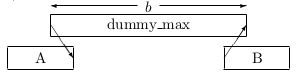
\includegraphics[width=5cm]{max_dur_1.png}}
            \hfill
            \subfloat[Expressing Maximum Elapsed time with Enveloping]
                    { 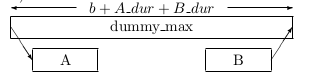
\includegraphics[width=5cm]{max_dur_2.png}}\\
            \vfill
            \centering
            \subfloat[Compact notation of possible combinations]
                    { 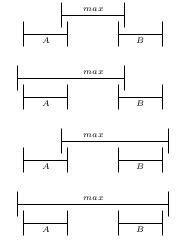
\includegraphics[width=4cm]{max_diff.png}}
                \caption{}
                \label{fig:maximum_compact}
        \label{fig:maximum}
        \end{figure}

        
        Figure \ref{fig:minimum} shows how to represent the minimum difference constraint \(x-y>=b\) (i.e, the minimum time allowed for \(x\) to follow \(y\)). Notice that when expressing a minimum constraint, regardless of the representation, the direction of the arrows is from the first action to the start of the durative (potentially dummy) action, and from the end of durative (potentially dummy) action to the second action (i.e.\ By manipulating the preconditions, invariants and effects of actions to enforce the order). Note that, with the minimum constraint, there is no maximum ensured. The second action can occur at any point after the first once it passed the minimum (or never).

        \begin{figure}[h]
                \subfloat[Expressing Minimum Elapsed time with Clipping]
                        { 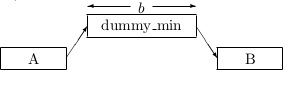
\includegraphics[width=5cm]{min_dur_1.png}}
                \hfill
                \subfloat[Expressing Minimum Elapsed time with Enveloping]
                        { 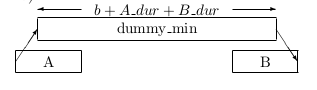
\includegraphics[width=5cm]{min_dur_2.png}}
                \vfill
                \centering 
                \subfloat[Compact notation of possible combinations]
                        { 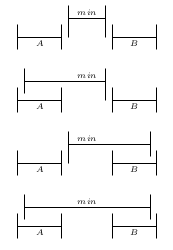
\includegraphics[width=4cm]{min_diff.png}}
                \caption{}
                \label{fig:minimum_compact}
        \label{fig:minimum}
        \end{figure}


        The more interesting cases would be when both constraints were to be modelled at the same time Figure \ref{fig:maxandmin}. 

        \begin{figure}[!]
            \centering    
            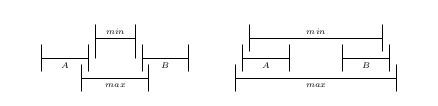
\includegraphics[width=11cm]{max_min.png}
            \caption{Expressing both Minimum and Maximum Time Between Actions in PDDL2.1}
             \label{fig:maxandmin}
        \end{figure}

        \subsubsection{Analysis of Representations}
        The two representation "clipping" vs "enveloping", though syntactically equivalent, are not always semantically equivalent.
        Some domains would correspond in its encoding to one representation but not to the other, even though, it would seem equivalent in some other domains. Further more, in the envelop representation, the duration of the durative action (potentially dummy) seems to depend on the duration of the actions it envelops (namely, the content actions). This results in a tight coupling between the content actions and the constraint they are fulfilling. Whilst in clipping, this is not the case. In clipping, planning and scheduling problems do not interact in a complex manner, resulting for both problems to be loosely coupled.
        To push it even further, what if those durative (potentially dummy) actions are not really dummy at all. What if they are actions with a specific duration, conditions and effects, that the content actions can only be executed during them. In this case, the problem just looks like a maximum constraint problem, but in fact it is not a maximum problem at all. In this case we have very little control over the duration of the enveloping action. The specific arrangement of those actions, envelope and content, need to be ensured by the planner as not to break any temporal constraint.

         In summary, translating the problem from one representation to the other highly depends on the semantics of the domain and are not always possible.
        
        On the bright side, we have just made clear when exactly, the planning and scheduling problems in temporal planning, are too tightly coupled to separate, where the logical constraints and the temporal constraint interact and can not be solved separately. This gives CRIKEY and similar systems the inspiration for when it would make sense to separate the problems and solve each of it alone, and to when the separation would effect the problem description in essence, and it would be required to find more clever ways to solve both together.



\chapter{CRIKEY} \label{crikey}
   This chapter focuses on how CRIKEY, a planner that separates the logical and temporal reasoning, tackles the separation of the sub-problems 

    Section~\ref{motivation} provides some insight on a predecessor system, problems with it and what motivates CRIKEY.
    Section~\ref{tech} provide some technical specification on the planning and scheduling technologies used at the heart.
    Section~\ref{workings} overview of the system architecture, explanation of how and when it separates the problems when possible, how it detects the coupling of the problems, and how it deals with it.
    
    \section{motivation} \label{motivation}
    % review the system that was developed before crikey and decribe where the limitation was.Also the architecture of the system could be here
    A system was developed in \citep{Halsey2003TemporalPW} for separating out the temporal and logical reasoning requires in temporal planning. Figure \ref{architecture} summarizes the main idea of the system. Given a temporal domain and problem description in PDDL2.1. A translator separates out the temporal aspects translating it into a PDDL classical planning problem and domain that preserves the key temporal relations. 
    The temporal information about actions duration are stored in a separate file. The translator used was the same as in LPGP \citep{Long:2003:EGF:3036969.3036977}. It splits a durative action into three instantaneous actions, modelling the at start conditions and effects, invariants and at end conditions and effects respectively. Later, the translated PDDL problem was solved with a classical planner producing a totally ordered plan.
    From the totally ordered plan, a partially ordered plan is lifted and fed, together with the duration file, separated at the begging, into a Simple Temporal Network. This schedules the plan by calculating relative and actual timing of actions. The product is a Temporal Plan.

    \begin{figure}[h]
        \centering    
        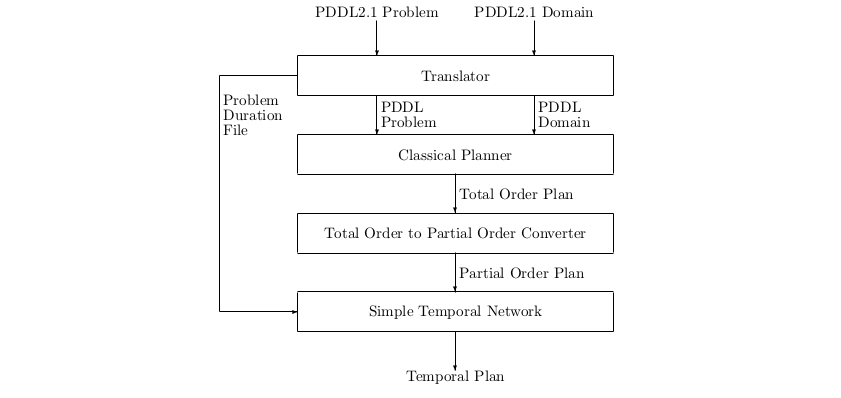
\includegraphics[width=15cm]{architecture.png}
        \caption{An Architecture for Separating Planning and Scheduling}
         \label{fig:architecture}
    \end{figure}
    
    This system always separates the planning and scheduling problem and solves each sub problem independently, as proposed in chapter~\ref{temporal_planning}. This turns out to be a good idea for a variety of domains (including all problems in International Planning Completion 2002). In these domains the solution plan could always be sequentialised (i.e.\ executed one action after the other). Concurrency was an optimization choice of the planner in case actions don't interfere. Yet, in those domains there was no concurrency enforced by the domains itself. In those domains, the temporal and logical constraints are loosely coupled and the problems do not deeply interact. 

    However, Some domains exist where this is not the case. Where it is necessary to perform some actions in parallel, and where the choice of actions depends on both their logical and temporal merits. In such domains the planning and scheduling problems are tightly coupled in the manner demonstrated in chapter~\ref{temporal_planning}. In these domains, the planner of predecessor of CRIKEY, would produce plans that the scheduler can not schedule. The un-schedulable plans comes from temporal constraint in the problem that are not met. The planner here lacks any temporal knowledge, and only makes its choices based on the logical constraints.

    This is where CRIKEY comes. CRIKEY basically inherits the same basic architecture for separating and solving the planning and scheduling problems independently when possible. Moreover, it always tries to detect cases where the problems are tightly coupled and solves them together. Details on how CRIKEY detects those cases and what does it do when it finds them are in the main focus of this chapter.

    \section{Technical Specification} \label{tech}
    CRIKEY planner was implemented in java.
    The planning algorithm implemented in CRIKEY is forward chaining heuristic planner.
    The implementation is based very closely on MetricFF \citep{hoffmann:ecai-02}.
    As in MetricFF, it uses a relaxed plan length as a heuristic, helpful actions (which appear in the first layer of the relaxed plan) to aid its action selection and performs Enforced Hill-Climbing.
    Unlike MetricFF, upon finding a plateau in the search space, it performs Best First Search to exit the plateau.
    This means expanding the same states as FF at the start, but if no exit found, will try those states that move away from the goal.

    \subsection{Action Splitting} \label{split}
    CRIKEY, separates the durative actions (when necessary) into two instantaneous actions.
    At start and at end instantaneous actions.
    % During the construction of the relaxed plan
    Invariants of the durative actions, become preconditions of the start and end spontaneous actions. Unless that invariant was achieved by the at start effects of the durative actions, it only becomes a condition of the end spontaneous action. For each state, the planner keeps a list of invariants that holds in that state. Actions that delete an invariant are considered inapplicable in this state. When an action is chosen, its invariants are either added to (if it was a start action) or removed from (if it was an end action) the invariants list.

    Another list keeps track of semi-complete actions. Those that their start action has been chosen, yet the end action is not. A final state could only be achieved if this list is empty and the goal is reached. The start actions are given a cost equal to its duration and end actions are given a small tolerance value (to motivate their selection in case they were not selected for some useful effect).

    This list also comes in handy during the extraction of the heuristic value from the relaxed plan. If during graph plan generation, a start action was chosen for its desired effect, but not its end action, only the start action will show in the relaxed plan. However if later, during plan relaxed plan extraction this start action was selected, then its end action needs to also be selected, increasing the size of the relaxed plan by one.

    CRIKEY does not allow negative conditions in a durative action.

    \section{The Workings of CRIKEY} \label{workings}
    As discussed in chapter~\ref{temporal_planning}, when a sequence of content actions needs to be completed before another set of enveloping actions do, is exactly when caution needs to be taken in their selection and ordering. If there not enough time to execute content actions during the enveloping actions we risk producing an unscheduled plan. CRIKEY, avoids this risk by looking for "potential envelopes". Here we are looking for actions that allow other actions to only execute during their duration.

    The detection happens in two different place in the algorithm with very similar reasoning. Once during the construction of the relaxed plan graph and extraction of the relaxed plan (during calculation of the heuristic). And another, during the actions selection. When a durative action is identified as a "potential envelops" . The durative action is then split into a start and end instantaneous actions (as described in the previous section). When an durative actions is clearly not an envelope, the durative action is condensed into one instantaneous action (with effects combined and the conditions are the at start conditions combined with any invariants unsatisfied by the at start effects). If the "potential envelope" action is later selected by the FF planner, on adding the start action, a mini-scheduler is associated with it to ensure there is enough time for any potential content actions to execute during the enveloping action. A content action is only selected if there is enough time for it to execute with the consideration of any other content actions already selected within the envelope. Once the envelope end action is selected the mini-scheduler is discarded.


    \begin{figure}[h]
        \centering    
        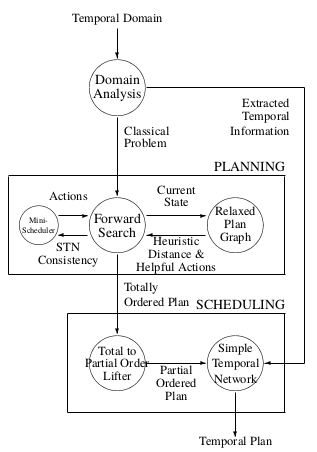
\includegraphics[width=6cm]{architecture_crikey.png}
        \caption{Architecture of CRIKEY}
         \label{fig:arch_crikey}
    \end{figure}



        \subsubsection{Detecting Envelops}
        During the construction and extraction of the relaxed plan, delete lists are ignored. A durative action is considered safe and condensed into a single action, if all of their at end conditions are satisfied by at start the add effect, Figure \ref{fig:none_env_rpg}. Otherwise, when there is an at end cond unsatisfied by the at start effects, it is considered an envelop, and split into start and end actions.
         \begin{figure}[h]
            \centering    
            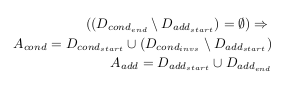
\includegraphics[width=6cm]{env_RPG.png}
            \caption{A Durative Action D is condensed into an Instantaneous Action A}
             \label{fig:none_env_rpg}
        \end{figure}


        During the action selection, delete lists needs to be taken into account. Similar reasoning is used to identify none envelope cases, Figure \ref{fig:none_env_selection}.
          \begin{figure}[h]
            \centering    
            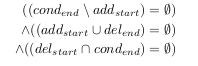
\includegraphics[width=5cm]{env_selection.png}
            \caption{When a durative action is considered none envelop}
             \label{fig:none_env_selection}
        \end{figure}

         Follows is the reasoning presented at \citep{crikey_1}. "s1,s2 and s3 are three states immediately before a start of the action, immediately after and immediately after the end of the action. An action applicable in s2 but not s1 must have been achieved by the at start add effect (since there is no negative conditions it could not have been achieved by an at start delete effect). Taking it further, there are no actions the could be applied in s2 and not s3 which could not have been applied in s1, apart from those achieved by the at start add effects and then deleted by the at end delete effects. Alternatively, an action could be achieved by the at start effect, and the effects of this action needed to achieve the end conditions. They are called potential envelopes since there is no effort (at this moment) to find out if there are any content actions that must go in these envelops"

          To recap, actions which allow other actions to happen only during their duration is what we are looking for. This formalization of these enveloping actions is described in figure.
          \begin{figure}[h]
            \centering    
            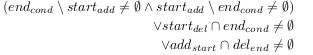
\includegraphics[width=8cm]{envelops.jpg}
            \caption{Envelops Formalization}
             \label{fig:envelops}
        \end{figure}


        \subsubsection{The Mini-scheduler}
        Each mini-scheduler associated with an envelope action, consists of a Simple Temporal Network, a list of content actions that need to fit inside the envelope and their ordering. The mini scheduler and the main scheduler in CRIKEY both use the same algorithm. After an enveloping start action is selected, the mini-scheduler makes sure to only select a content action if the STN is consistent. Meaning there will be enough time to execute the content action within the envelope. Content actions that are deemed inapplicable by the STN, are pruned. Figure \ref{fig:algorithm} shows the pseudo code describing the mini-scheduler.
        \begin{figure}[h]
            \centering    
            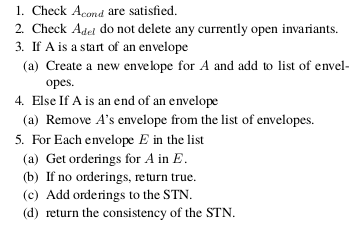
\includegraphics[width=8cm]{sched_algorithm.png}
            \caption{Algorithm to decide whether an action A is applicable}
             \label{fig:algorithm}
        \end{figure}

        \subsubsection{The Scheduler}
        After the partial order lifter (modified version of \citep{rintegrating})  produces a partial orders plan. It is passed through a Simple Temporal Network that uses Floyd-Warshall's algorithm to compute the actual timing of actions, producing a temporal plan.

    \section{Conclusion} 
    Crikey was the first planner to successfully managed to generate valid temporal plans by separating the logical and temporal reasoning. It was demonstrated how Crikey managed to do that. It might have suffered from several limitation. Although it will not find an optimal plan (i.e. one that exploits all concurrency possible) it is complete and sound. Crikey opened the door for an area of research that follow. Some of the direct predecessors of CRIKEY is POPF and CRIKEY3.


%%% End of seminar %%%


\listoffigures

\bibliographystyle{plainnat}
\bibliography{seminar}


\end{document}

